\documentclass[dissertation.tex]{subfiles}
\begin{document}

\chapter{Large-scale subjective evaluation}

\cite{pearce2001towards} addresses difficulty in quantitative evaluation,
suggesting the use of a learned critic in a manner similar to GANs
\cite{goodfellow2014generative}. In a later report,
\cite{pearce2002motivations} attribute difficulty in evaluation due to lack
aim: algorithmic composition, design of compositional tools, and computational
modelling of musical styles or music cognition all have different motivations
and should thus be evaluated differently.

Following advice of \cite{pearce2002motivations}, we identify our key
motivation as algorithmic composition: generation of novel compositions.
To evaluate our success, we employ a subjective evaluation method.

\cite{ariza2009interrogator} criticizes a musical Turing test as providing little data about
how to improve the system, suggesting that listener studies using music experts
may be more insightful.

\section{Evaluation framework design}

\subsection{Software architecture}

The frontend utilizes React and Redux, allowing us to collect fine-grained user
action data. Azure App Service is used to host an Express web-service which
randomizes experimental questions and collects responses. The data is stored to
Azure Data Storage and processed in batch MapReduce using Azure HDInsight.

\subsection{User interface}


The landing page for \url{http://bachbot.com/} is shown in \cref{fig:bachbot-front-page}.

\begin{figure}[htpb]
  \centering
  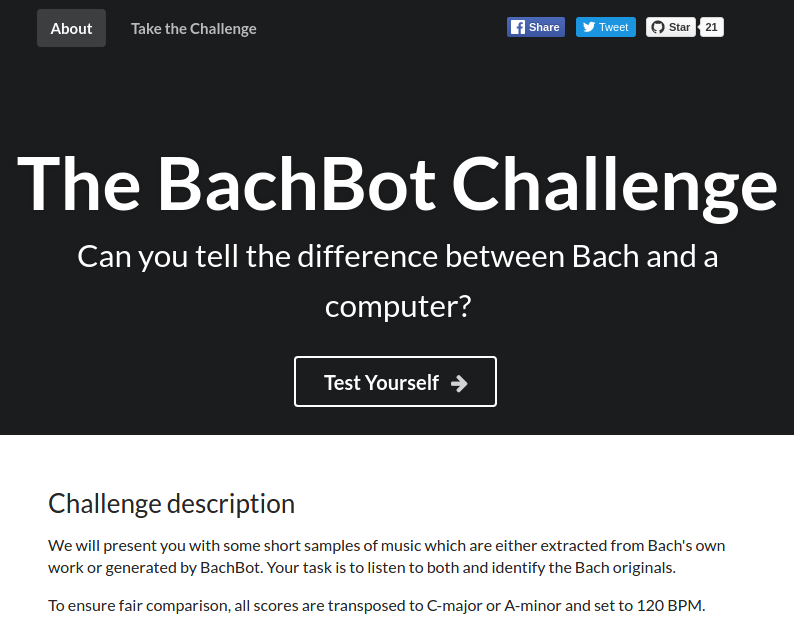
\includegraphics[width=1.0\linewidth]{Figures/bachbot-front-page.png}
  \caption{The first page seen by a visitor of \url{http://bachbot.com}}
  \label{fig:bachbot-front-page}
\end{figure}

Clicking ``Test Yourself'' redirects the participant to a user information form
(\cref{fig:user-info-form}) where users self-report their age
group prior music experience into the categories shown.

\begin{figure}[htpb]
  \centering
  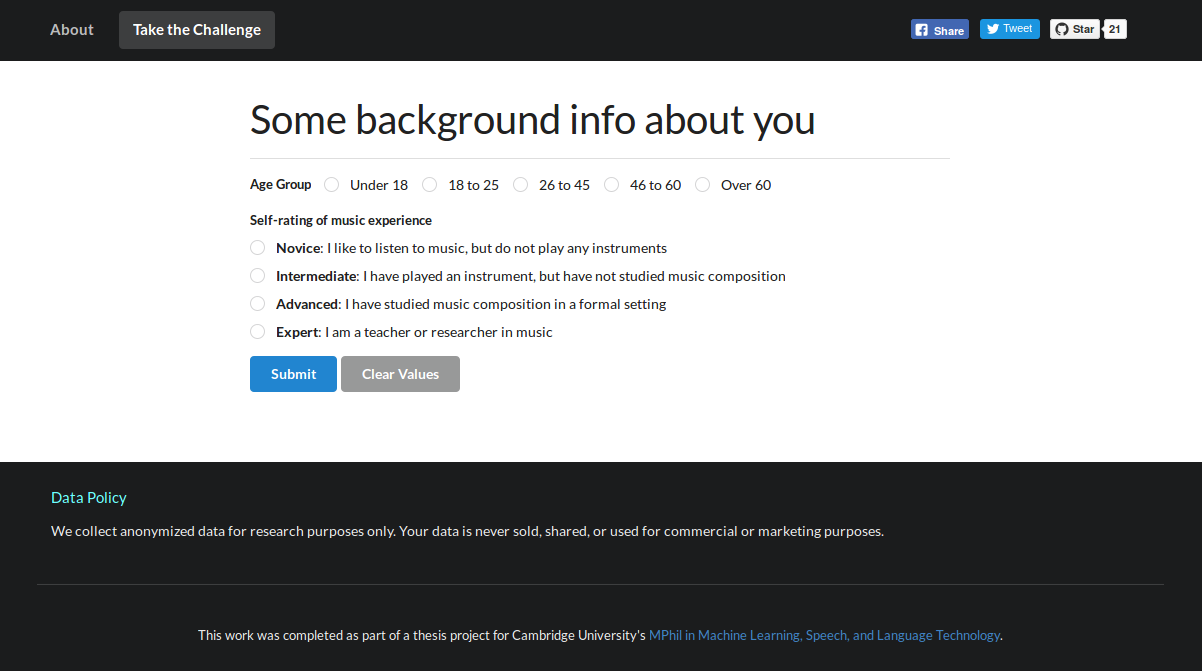
\includegraphics[width=1.0\linewidth]{Figures/user-info-form.png}
  \caption{User information form presented after clicking ``Test Yourself''}
  \label{fig:user-info-form}
\end{figure}

After submitting the background form, users were redirected to the question
response page shown in \cref{fig:question-screen}. This page contains two
audio samples, one extracted from Bach and one generated by BachBot, and users
were asked to select the sample which sounds most similar to Bach. Users were
asked to provide five consecutive answers and then the overall percentage
correct was reported.

\begin{figure}[htpb]
  \centering
  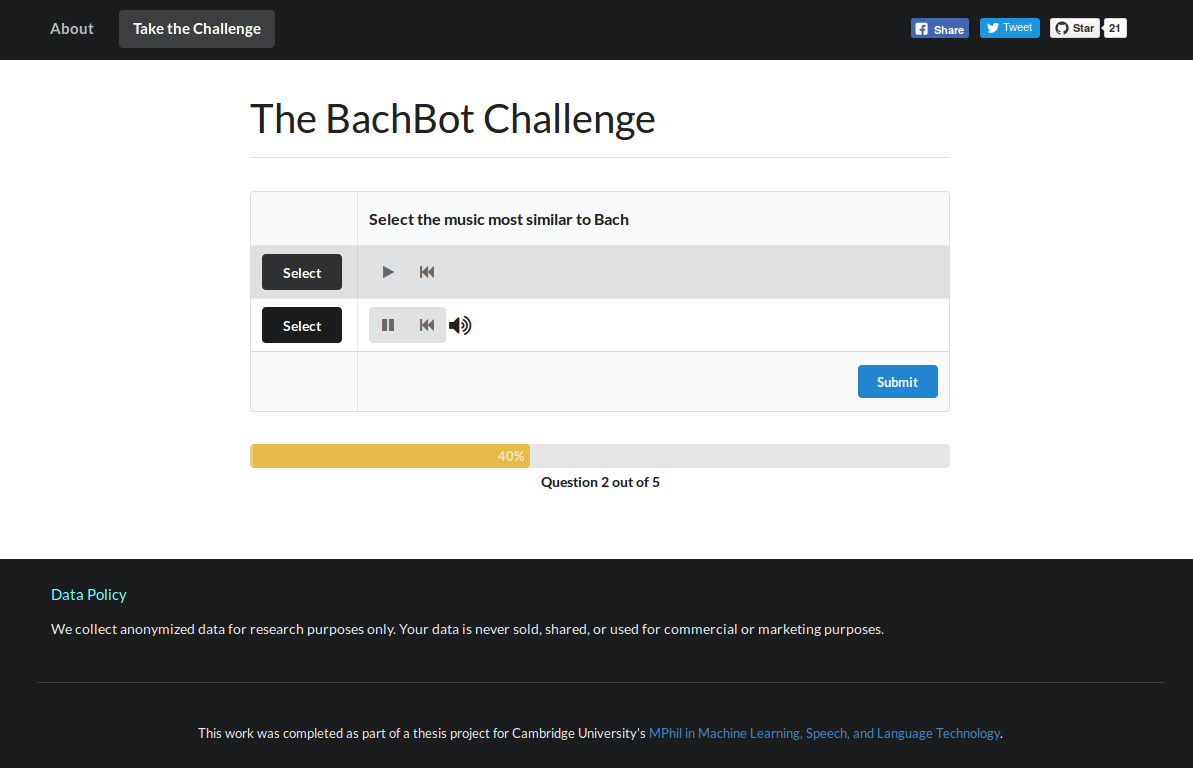
\includegraphics[width=1.0\linewidth]{Figures/question-screen.png}
  \caption{Question response interface used for all questions}
  \label{fig:question-screen}
\end{figure}

\subsection{Question generation}

Questions were generated for both harmonizations (using the same abbreviations
as defined in \todo{ref}) as well as original compositions (denoted SATB as all parts
are generated). For each question, a random chorale was selected without
replacement from the corpus and paired with a corresponding harmonization.
SATB sampls were paired with chorales randomly sampled from the corpus. The
five question answered by any given participant were comprised of one S/A/T/B
question chosen at random, one AT question, one ATB question, and two original
compositions. See
\cref{tab:bachbot-com-question-distribtion} for details.

\begin{table}[htpb]
  \centering
  \begin{tabular}{lrr}
    \toprule
    Question Type & \# Questions &  Expected \# responses / participant \\
    \midrule
    S        & 2  & 0.25 \\
    A        & 2  & 0.25 \\
    T        & 2  & 0.25 \\
    B        & 2  & 0.25 \\
    AT       & 8  & 1 \\
    ATB      & 8  & 1 \\
    SATB     & 12 & 2 \\
    \bottomrule
  \end{tabular}
  \caption{Composition of questions on \url{http://bachbot.com}}
  \label{tab:bachbot-com-question-distribtion}
\end{table}

\section{Results}

\subsection{Participant backgrounds and demographics}

We recieved a total of \todo{FILL THIS IN LAST} responses from \todo{FILL THIS
IN LAST} different countries. As evidenced by \cref{fig:user-geographics},
our participant is diverse and includes participants from six different continents.
\cref{fig:user-demographics} shows that while the majority of our participants
are between $18-45$ and have played an instrument, more than $20\%$\todo{FIX NUMBER LAST}
have either formally studied or taught music theory.

\begin{figure}[htpb]
  \centering
  \begin{subfigure}[b]{0.98\textwidth}
    \centering
    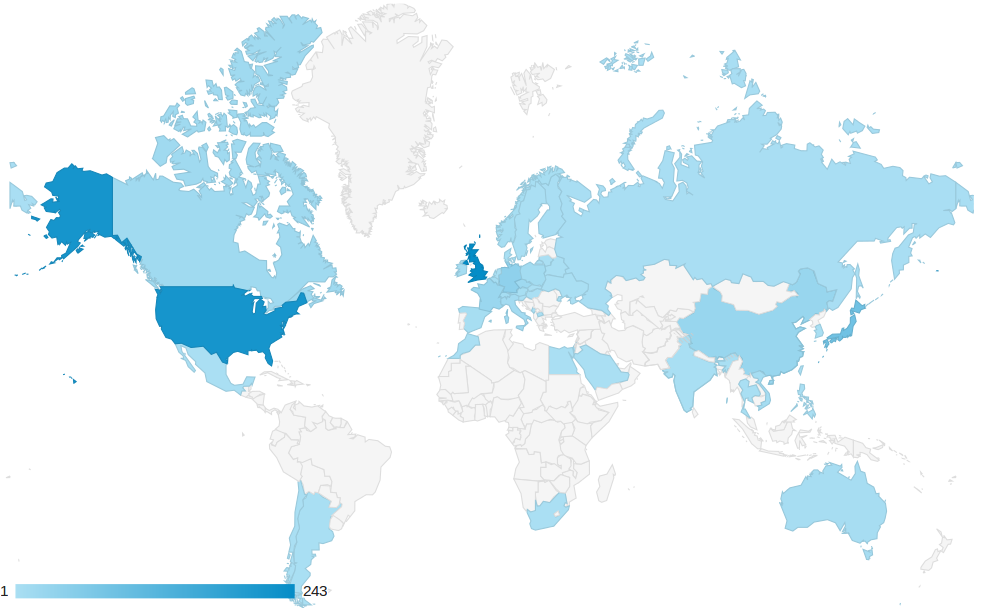
\includegraphics[width=0.85\linewidth]{Figures/participants-by-country.png}
  \end{subfigure}
  \begin{subfigure}[c]{0.55\textwidth}
    \centering
    \hspace{-1cm}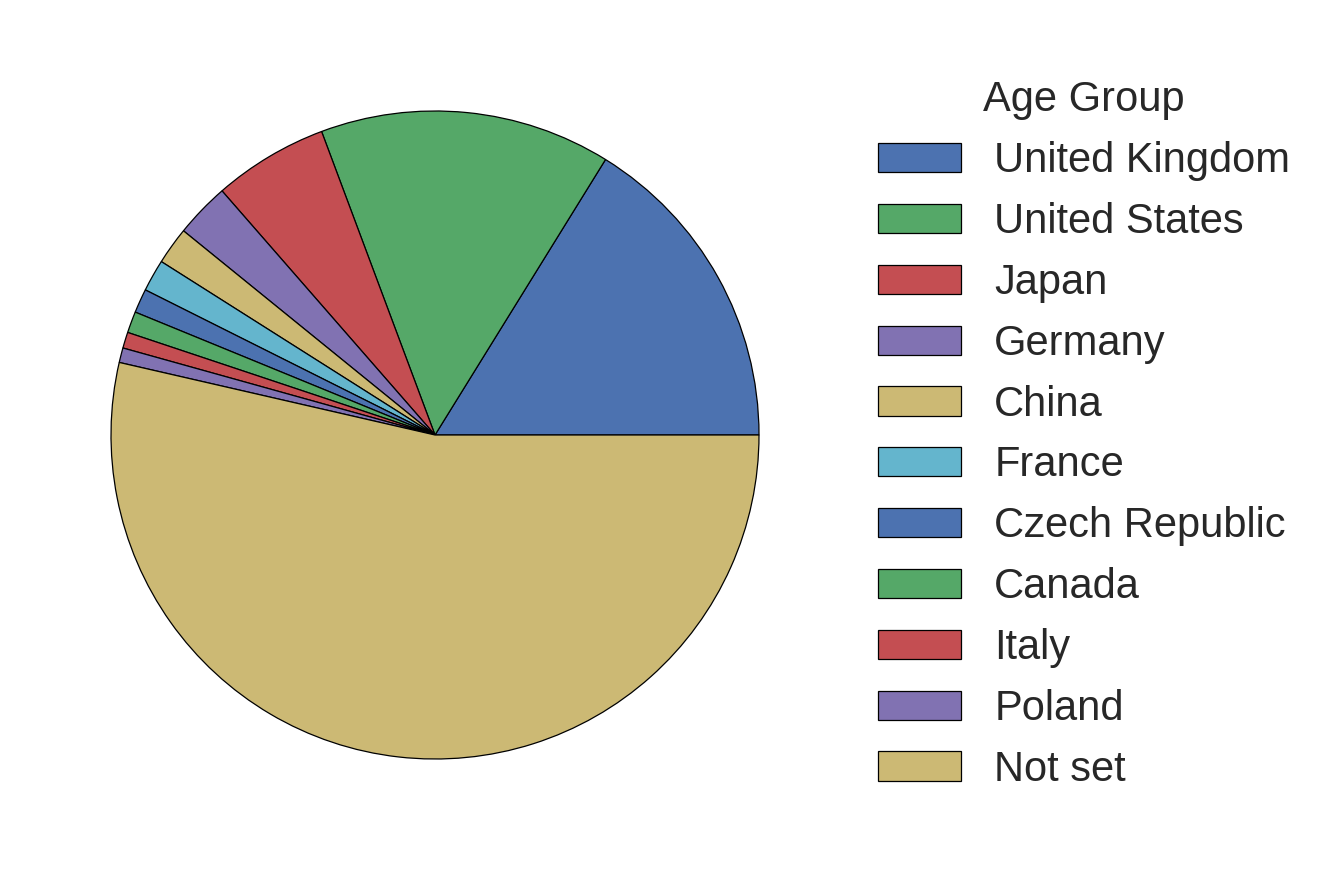
\includegraphics[width=3in]{Figures/user-demographics-pie.png}
  \end{subfigure}
  \begin{subfigure}[c]{0.44\textwidth}
    \centering
    \begin{tabular}{lrr}
\toprule
Country        &  Responses       &  Proportion \\
\midrule
UK             &       243 &            16.0\% \\
US             &       218 &            15.0\% \\
Japan          &        86 &             6.0\% \\
Germany        &        41 &             3.0\% \\
China          &        28 &             2.0\% \\
France         &        24 &             2.0\% \\
Czechia        &        18 &             1.0\% \\
Canada         &        16 &             1.0\% \\
Italy          &        12 &             1.0\% \\
Poland         &        11 &             1.0\% \\
Not set        &       805 &            54.0\% \\
\bottomrule
\end{tabular}

  \end{subfigure}
  \caption{Geographic distribution of participants}
  \label{fig:user-geographics}
\end{figure}

\begin{figure}[htpb]
  \centering
  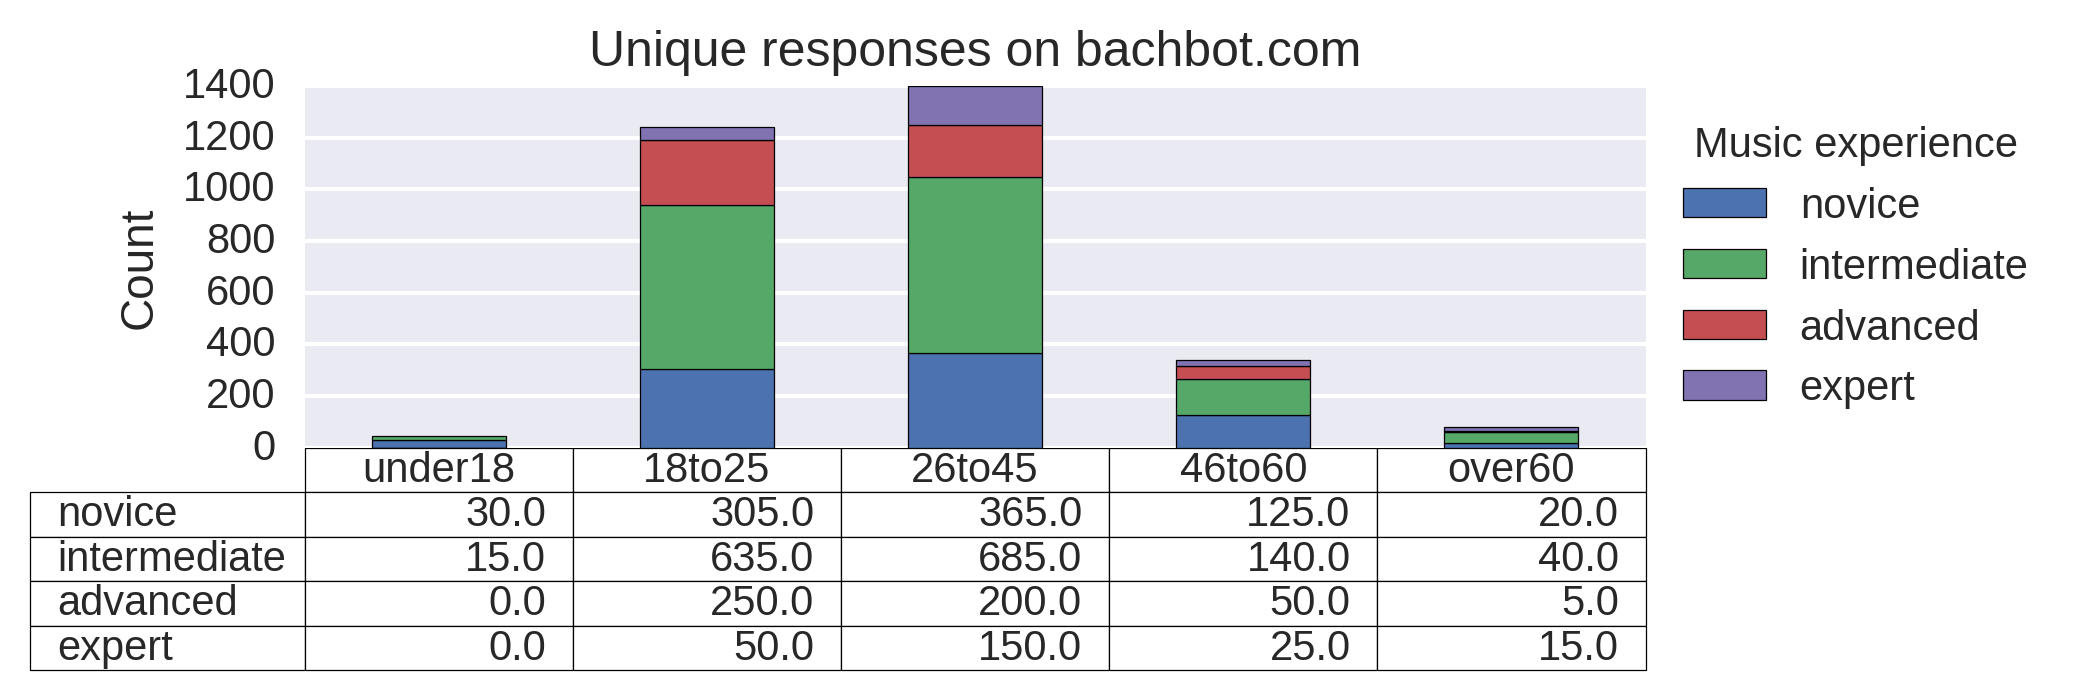
\includegraphics[width=\textwidth]{Figures/responses-ageGroup-musicExperience.png}
  \caption{Demographics of participants}
  \label{fig:user-demographics}
\end{figure}

\subsection{BachBot's performance results}

\todo{\cref{fig:responses-mask} suggests performance is weakest on
  harmonizations. Unsurprising because we only do 1-best and don't account
  for future. Bidirectional LSTM or N-best lattice search (reference marcin)
  would do better}

\cref{fig:responses-mask} shows the performance of BachBot on various question
types. It shows that $59\%$\todo{VERIFY LAST} of participants could correctly
identify original Bach from BachBot's generated music. As the baseline method
of randomly guessing between the two choices in \cref{fig:question-screen}
achieves $50\%$, our findings suggest that {\bf the average participant has only a
$9\%$\todo{VERIFY LAST} better chance than randomly guessing when
distinguishing Bach from BachBot correctly}.

\begin{figure}[htpb]
  \centering
  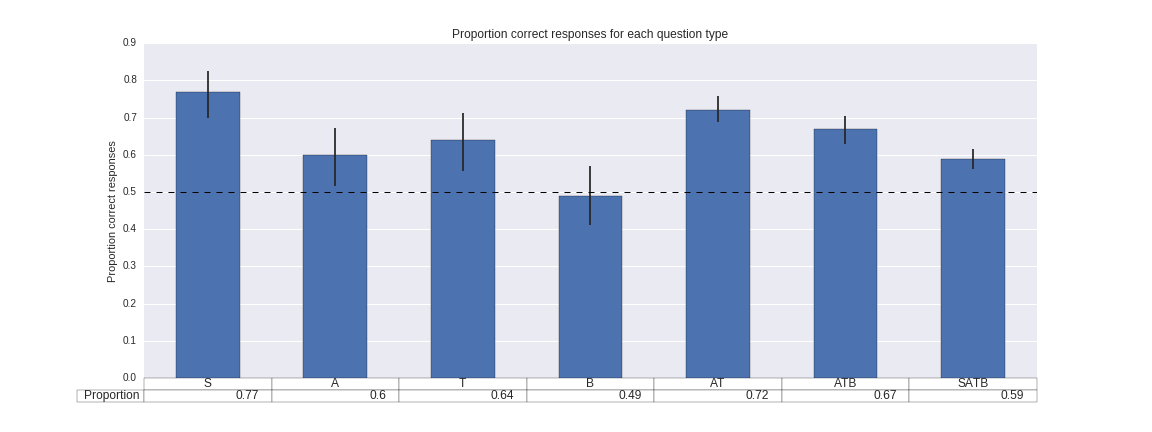
\includegraphics[width=0.8\textwidth]{Figures/responses-mask.png}
  \caption{Figures/responses-Mask}
  \label{fig:responses-mask}
\end{figure}

\cref{fig:responses-mask} also shows that participants had more trouble
discriminating entire compositions (SATB) than harmonizations (AT, ATB) where a
subset of the parts have already been given. While this may seem
counterintuitive, recall that the model in \todo{reference} is uni-directional
and does not account for any future constraints on other parts. We made
this design decision intentionally because one of our requirements was sampling
the model for novel compositions. However, since harmonization tasks provide
the full past and future context for other parts, they effectively impose constraints
on LSTM hidden state dynamics. We expect methods which account for both future and past
context (e.g. using the output sequence from a bidirectional RNN\todo{cite} inputs)
to mitigate this problem, which we leave for future work.

When only a only single part is composed by BachBot, we find the results vary significantly
across different parts. Composing the soprano part proved to be the easiest to
discriminate, an unsurprising result given that in chorale style music soprano parts
are responsible for the melody\todo{cite}. Composing the alto and tenor parts achieved
similar performance as composing all four parts, a result which may also be caused by
not accounting for future constraints on model outputs. Removing the bass proved
to be the most perceptually difficult to discern from real Bach.

In \cref{fig:responses-mask-musicExperience}, responses are further segmented
by music experience. Unsurprisingly, we find that the proportion of correct responses
correlates positively with experience.

\begin{figure}[htpb]
  \centering
  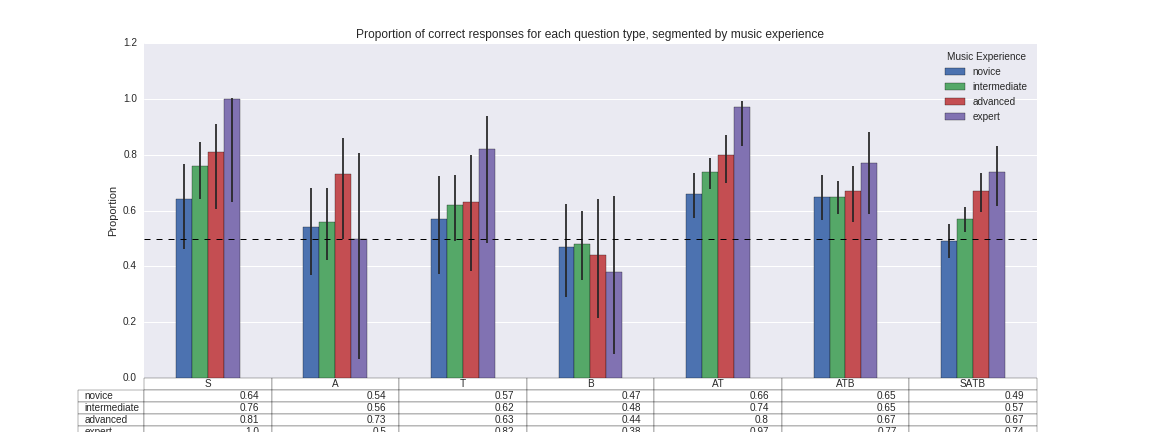
\includegraphics[width=1.0\textwidth]{Figures/responses-mask-musicExperience.png}
  \caption{Figures/responses-mask-MusicExperience}
  \label{fig:responses-mask-musicExperience}
\end{figure}

\begin{figure}[htpb]
  \centering
  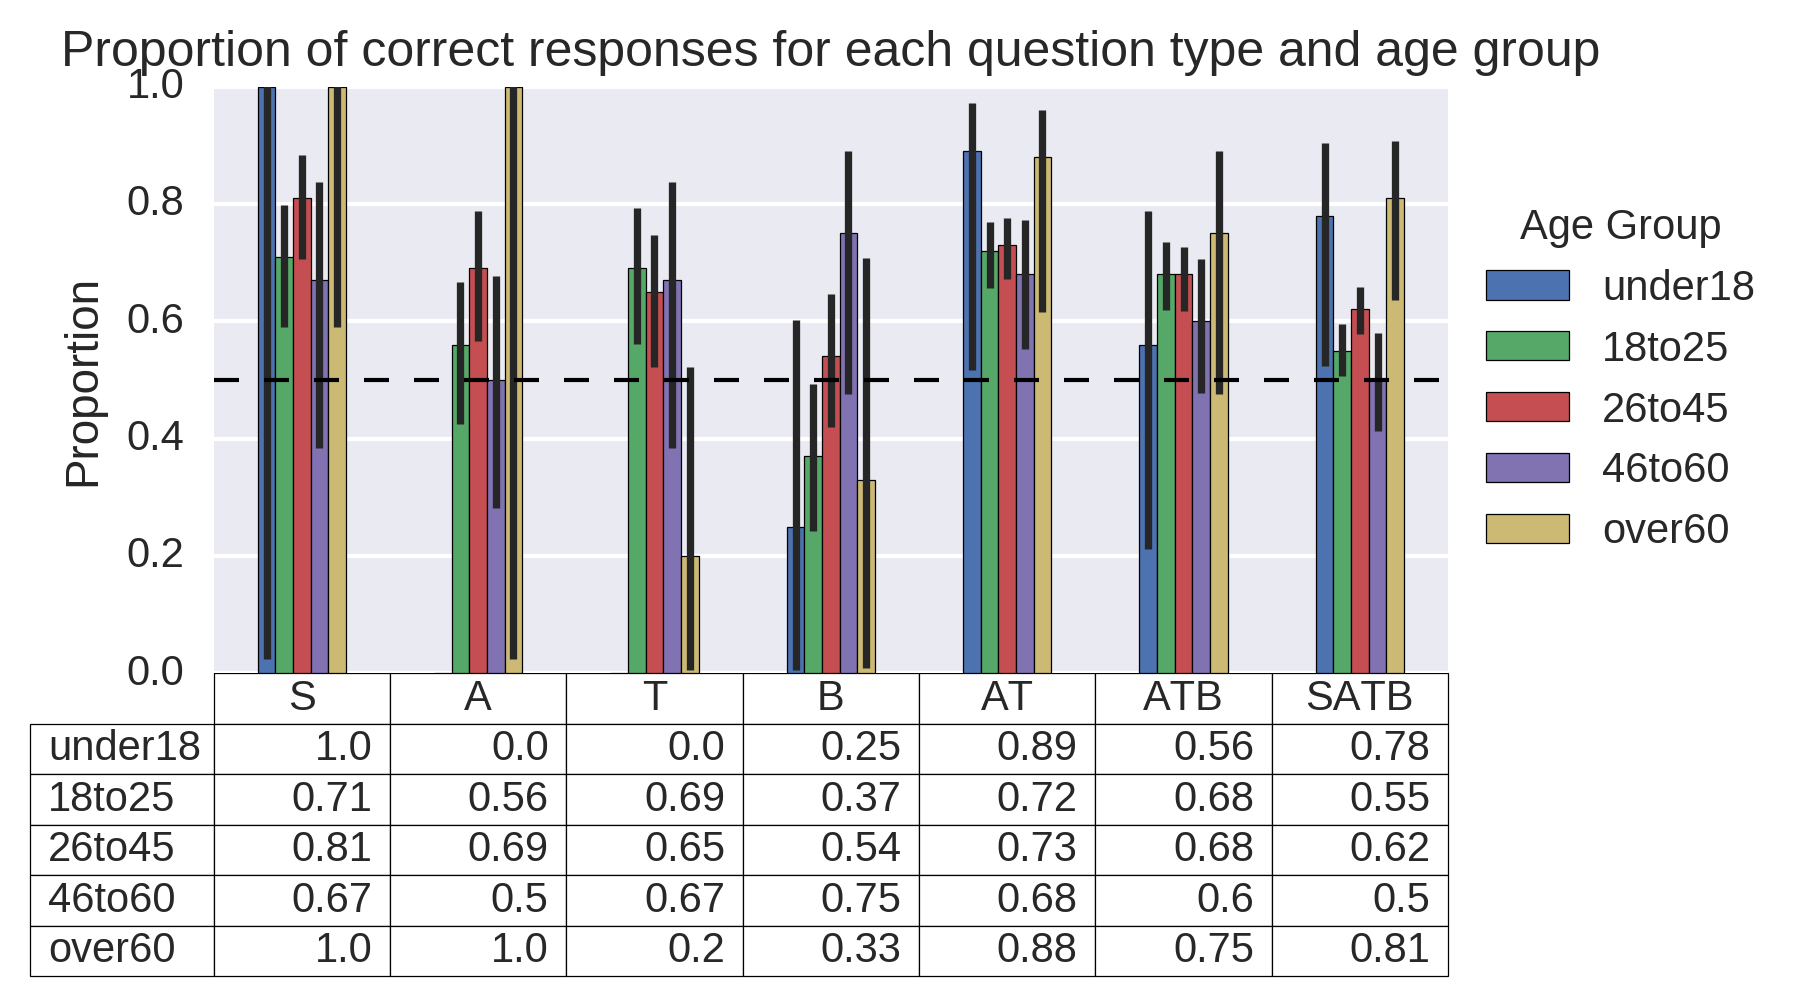
\includegraphics[width=1.0\textwidth]{Figures/responses-mask-agegroup.png}
  \caption{Figures/responses-mask-Agegroup}
  \label{fig:responses-mask-agegroup}
\end{figure}

\begin{figure}[htpb]
  \centering
  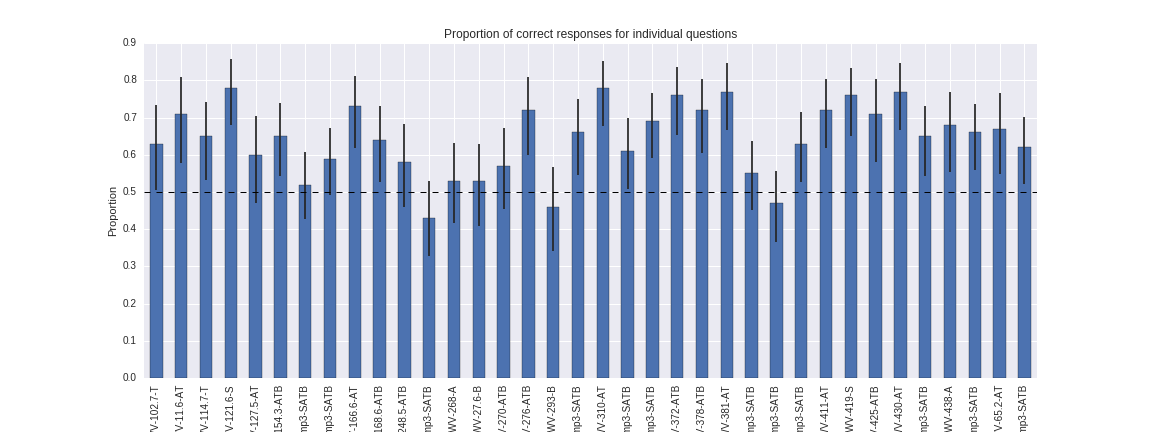
\includegraphics[width=0.8\linewidth]{Figures/responses-name.png}
  \caption{Proportion of correct responses broken down by individual questions.}
  \label{fig:responses-name}
\end{figure}

\cref{fig:responses-name} shows the proportion correct for each question.
Encouragingly, it shows that $41.7\%$\todo{VERIFY LAST} of the SATB pairs were not
statistically different than baseline, suggesting that \textbf{while not always
consistent BachBot is capable of composing music which the average participant
cannot discern from actual Bach}.

\todo{Have Mark analyze bad examples in \cref{fig:responses-name}}

\section{User feedback}

The modulations and part writing were the giveaway for me (and once or twice the phrasing)

Got 5/5. The trick is to listen for the unnatural pauses at regular intervals.

Cool project, I scored 100\% so I'm quite pleased with myself ;o) I do
play an instrument although I'm not classical trained. If I had an
inkling to why I could choose the background phrasing of the Bach
pieces is far more elegant than the computer generated pieces.

@samim @feynmanliang really impressive! If I didn't know about counterpoint that quiz would've stumped me



\printbibliography

\end{document}
